\documentclass[
	11pt, 
	%t, % Uncomment to vertically align all slide content to the top of the slide, rather than the default centered
	%aspectratio=169, % Uncomment to set the aspect ratio to a 16:9 ratio which matches the aspect ratio of 1080p and 4K screens and projectors
]{beamer}

\usepackage{graphicx}
\graphicspath{{Images/}{./}} % Specifies where to look for included images (trailing slash required)
\usepackage{pgfplots}

\usepackage{pgfplotstable}
\usepackage{booktabs}
\usepackage{algorithm}
\usepackage{amsmath}
\usepackage{algorithmic}
\usepackage{mathrsfs}
\usepackage{multicol}
\usepackage[many]{tcolorbox} 
\usepackage{booktabs} % Allows the use of \toprule, \midrule and \bottomrule for better rules in tables
\usepackage[latin1]{inputenc}
\usepackage{tikz}
\usepackage[most]{tcolorbox}

\usetikzlibrary{shapes,arrows,positioning}
\usetikzlibrary{positioning}
\definecolor{main}{HTML}{5989cf} 
\definecolor{sub}{HTML}{cde4ff} 
\newtcolorbox{boxD}{
    colback = sub, 
    colframe = main, 
    boxrule = 0pt, 
    toprule = 3pt, % top rule weight
    bottomrule = 3pt % bottom rule weight
}

%\usetheme{default}
\usetheme{AnnArbor}
%\usetheme{Antibes}
%\usetheme{Bergen}
%\usetheme{Berkeley}
%\usetheme{Berlin}
%\usetheme{Boadilla}
%\usetheme{CambridgeUS}
%\usetheme{Copenhagen}
%\usetheme{Darmstadt}
%\usetheme{Dresden}
%\usetheme{Frankfurt}
%\usetheme{Goettingen}
%\usetheme{Hannover}
%\usetheme{Ilmenau}
%\usetheme{JuanLesPins}
%\usetheme{Luebeck}
%\usetheme{Madrid}
%\usetheme{Malmoe}
%\usetheme{Marburg}
%\usetheme{Montpellier}
%\usetheme{PaloAlto}
%\usetheme{Pittsburgh}
%\usetheme{Rochester}
%\usetheme{Singapore}
%\usetheme{Szeged}
%\usetheme{Warsaw}

%----------------------------------------------------------------------------------------
%	SELECT COLOR THEME
%----------------------------------------------------------------------------------------

% Beamer comes with a number of color themes that can be applied to any layout theme to change its colors. Uncomment each of these in turn to see how they change the colors of your selected layout theme.

%\usecolortheme{albatross}
%\usecolortheme{beaver}
%\usecolortheme{beetle}
%\usecolortheme{crane}
%\usecolortheme{dolphin}
%\usecolortheme{dove}
%\usecolortheme{fly}
%\usecolortheme{lily}
%\usecolortheme{monarca}
%\usecolortheme{seagull}
%\usecolortheme{seahorse}
\usecolortheme{spruce}
%\usecolortheme{whale}
%\usecolortheme{wolverine}

%----------------------------------------------------------------------------------------
%	SELECT FONT THEME & FONTS
%----------------------------------------------------------------------------------------

%\usefonttheme{default} % Typeset using the default sans serif font
%\usefonttheme{serif} % Typeset using the default serif font (make sure a sans font isn't being set as the default font if you use this option!)
%\usefonttheme{structurebold} % Typeset important structure text (titles, headlines, footlines, sidebar, etc) in bold
%\usefonttheme{structureitalicserif} % Typeset important structure text (titles, headlines, footlines, sidebar, etc) in italic serif
\usefonttheme{structuresmallcapsserif} % Typeset important structure text (titles, headlines, footlines, sidebar, etc) in small caps serif

%------------------------------------------------

%\usepackage{mathptmx} % Use the Times font for serif text
\usepackage{palatino} % Use the Palatino font for serif text

%\usepackage{helvet} % Use the Helvetica font for sans serif text
\usepackage[default]{opensans} % Use the Open Sans font for sans serif text
%\usepackage[default]{FiraSans} % Use the Fira Sans font for sans serif text
%\usepackage[default]{lato} % Use the Lato font for sans serif text

%----------------------------------------------------------------------------------------
%	SELECT INNER THEME
%----------------------------------------------------------------------------------------

% Inner themes change the styling of internal slide elements, for example: bullet points, blocks, bibliography entries, title pages, theorems, etc. Uncomment each theme in turn to see what changes it makes to your presentation.

%\useinnertheme{default}
%\useinnertheme{circles}
\useinnertheme{rectangles}
%\useinnertheme{rounded}
%\useinnertheme{inmargin}

%----------------------------------------------------------------------------------------
%	SELECT OUTER THEME
%----------------------------------------------------------------------------------------

% Outer themes change the overall layout of slides, such as: header and footer lines, sidebars and slide titles. Uncomment each theme in turn to see what changes it makes to your presentation.

%\useoutertheme{default}
\useoutertheme{infolines}
% \useoutertheme{miniframes}
%\useoutertheme{smoothbars}
% \useoutertheme{sidebar}
% \useoutertheme{split}
% \useoutertheme{shadow}
% \useoutertheme{tree}
% \useoutertheme{smoothtree}

% \setbeamertemplate{footline} % Uncomment this line to remove the footer line in all slides
% \setbeamertemplate{footline}[page number] % Uncomment this line to replace the footer line in all slides with a simple slide count

% \setbeamertemplate{navigation symbols}{} % Uncomment this line to remove the navigation symbols from the bottom of all slides

%----------------------------------------------------------------------------------------
%	PRESENTATION INFORMATION
%----------------------------------------------------------------------------------------

\title[LSMT]{Log-Structured Merge-Tree} % The short title in the optional parameter appears at the bottom of every slide, the full title in the main parameter is only on the title page

\subtitle{Effective Data Structure for Memory Storage} % Presentation subtitle, remove this command if a subtitle isn't required

\author[MR \and FAT \and JI]{Mohammad Rahim \and Faihaj Alam Topu \and Jarif Islam} % Presenter name(s), the optional parameter can contain a shortened version to appear on the bottom of every slide, while the main parameter will appear on the title slide

\institute[BUET]
{
    Department of CSE\\
    Bangladesh University of Engineering \& Technology
}
%\textit{james@LaTeXTemplates.com}} % Your institution, the optional parameter can be used for the institution shorthand and will appear on the bottom of every slide after author names, while the required parameter is used on the title slide and can include your email address or additional information on separate lines

\date[\today]{CSE300 Presentation \\ \today} % Presentation date or conference/meeting name, the optional parameter can contain a shortened version to appear on the bottom of every slide, while the required parameter value is output to the title slide

%----------------------------------------------------------------------------------------

\begin{document}

%----------------------------------------------------------------------------------------
%	TITLE SLIDE
%----------------------------------------------------------------------------------------

\begin{frame}
	\titlepage % Output the title slide, automatically created using the text entered in the PRESENTATION INFORMATION block above
\end{frame}

%----------------------------------------------------------------------------------------
%	TABLE OF CONTENTS SLIDE
%----------------------------------------------------------------------------------------

% The table of contents outputs the sections and subsections that appear in your presentation, specified with the standard \section and \subsection commands. You may either display all sections and subsections on one slide with \tableofcontents, or display each section at a time on subsequent slides with \tableofcontents[pausesections]. The latter is useful if you want to step through each section and mention what you will discuss.

\begin{frame}
	\frametitle{Presentation Outline} % Slide title, remove this command for no title
	\begin{multicols}{2}
	   \tableofcontents % Output the table of contents (all sections on one slide)
	%\tableofcontents[pausesections] % Output the table of contents (break sections up across separate slides)
        \end{multicols}
\end{frame}

%----------------------------------------------------------------------------------------
%	PRESENTATION BODY SLIDES
%----------------------------------------------------------------------------------------

\section{Introduction}

\subsection{First Intro}

\begin{frame}
    \frametitle{A Brief Intro}
    \begin{columns} 
        \column{0.7\textwidth}
            Log-Structured Merge-Tree (Shortly known as LSM Tree) is a data structure with performance data structure that makes it very attractive to store data with high insert and update rates. \newline \newline
            It comprises of tree-like data structure with 2 or more levels: 
            \begin{enumerate}
                \item Memtable completely resided in memory
                \item SSTables stored in disk
            \end{enumerate}
        \column{0.3\textwidth}
            
\includegraphics[scale=0.5]{What.png}
    \end{columns}
\end{frame}

\subsection{Concepts}

\begin{frame}
    \frametitle{List of Concepts}
    LSM tree is based on 3 important concepts to optimize read and writes: \newline
    \begin{itemize}
        \item SSTables
        \item Memtable
        \item Compaction
    \end{itemize}
    
\end{frame}

\subsubsection{Memtable}

\begin{frame}
    \frametitle{Memtable}
    \begin{columns}
        \column{0.4\textwidth}
            \begin{tcolorbox}[colback=white, colframe=blue!50!black, arc=4mm]
                In-Memory DS
            \end{tcolorbox}
            \begin{tcolorbox}[colback=white, colframe=blue!50!black, arc=4mm]
                Write Cache
            \end{tcolorbox}
            \begin{tcolorbox}[colback=white, colframe=blue!50!black, arc=4mm]
                Self-Balancing Tree
            \end{tcolorbox}
        \column{0.6\textwidth}
             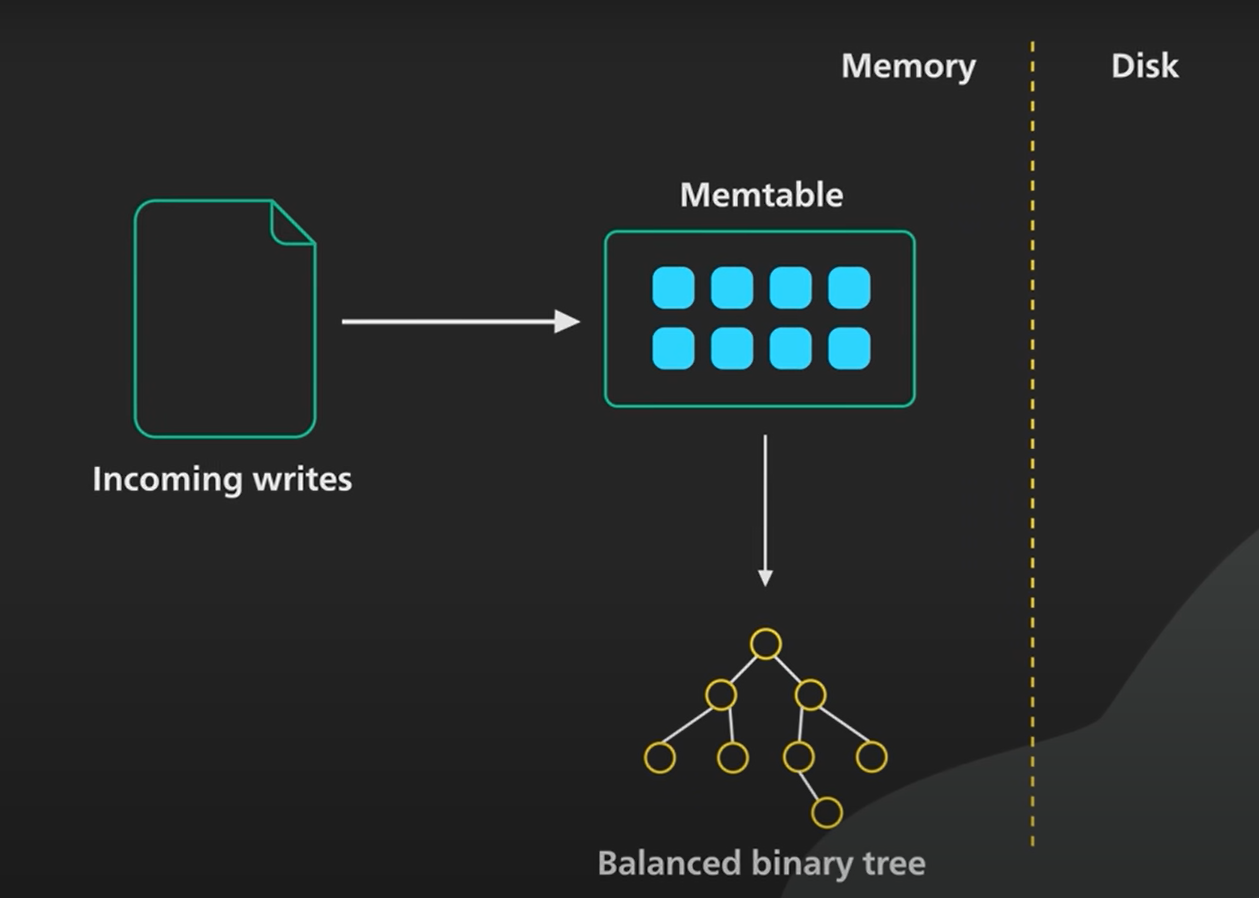
\includegraphics[scale=0.22]{Memtable.png}
    \end{columns}
    
\end{frame}

\subsubsection{SSTables}

\begin{frame}
    \frametitle{SSTables}
    \begin{columns}
        \column{0.4\textwidth}
            \begin{tcolorbox}[colback=white, colframe=blue!50!black, arc=4mm]
                Sorted String Table
            \end{tcolorbox}
            \begin{tcolorbox}[colback=white, colframe=blue!50!black, arc=4mm]
                Immutable
            \end{tcolorbox}
            \begin{tcolorbox}[colback=white, colframe=blue!50!black, arc=4mm]
                Key-Pair DS
            \end{tcolorbox}
        \column{0.6\textwidth}
             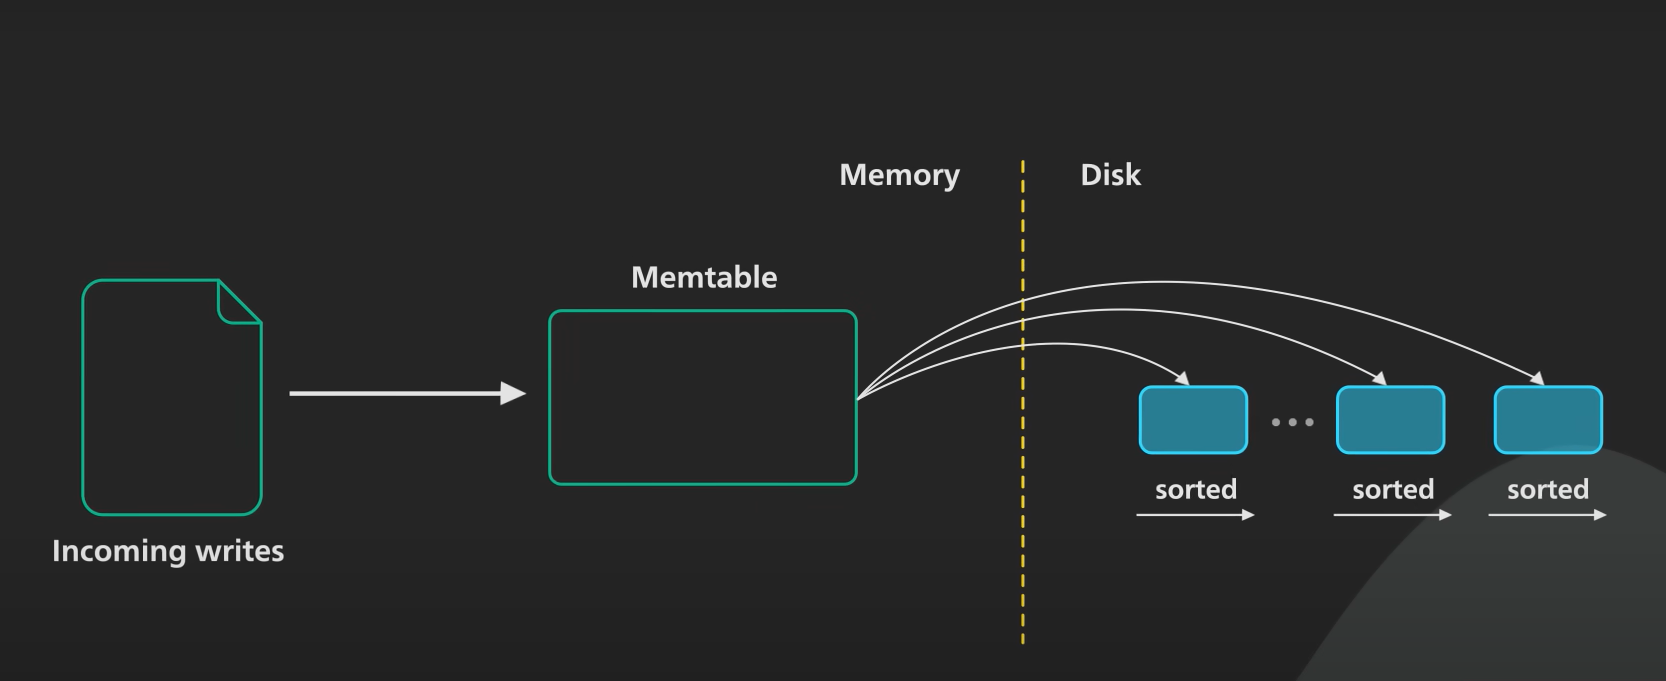
\includegraphics[scale=0.16]{SSTables.png}
    \end{columns} 
    
\end{frame}

\subsubsection{Compaction}

\begin{frame}
    \frametitle{Compaction}
    \begin{columns}
        \column{0.4\textwidth}
            \begin{tcolorbox}[colback=white, colframe=blue!50!black, arc=4mm]
                Removes Redundant Keys
            \end{tcolorbox}
            \begin{tcolorbox}[colback=white, colframe=blue!50!black, arc=4mm]
                Creates Compacted Merge Tree
            \end{tcolorbox}
            \begin{tcolorbox}[colback=white, colframe=blue!50!black, arc=4mm]
                Occurs Continuously Subsequently
            \end{tcolorbox}
        \column{0.6\textwidth}
             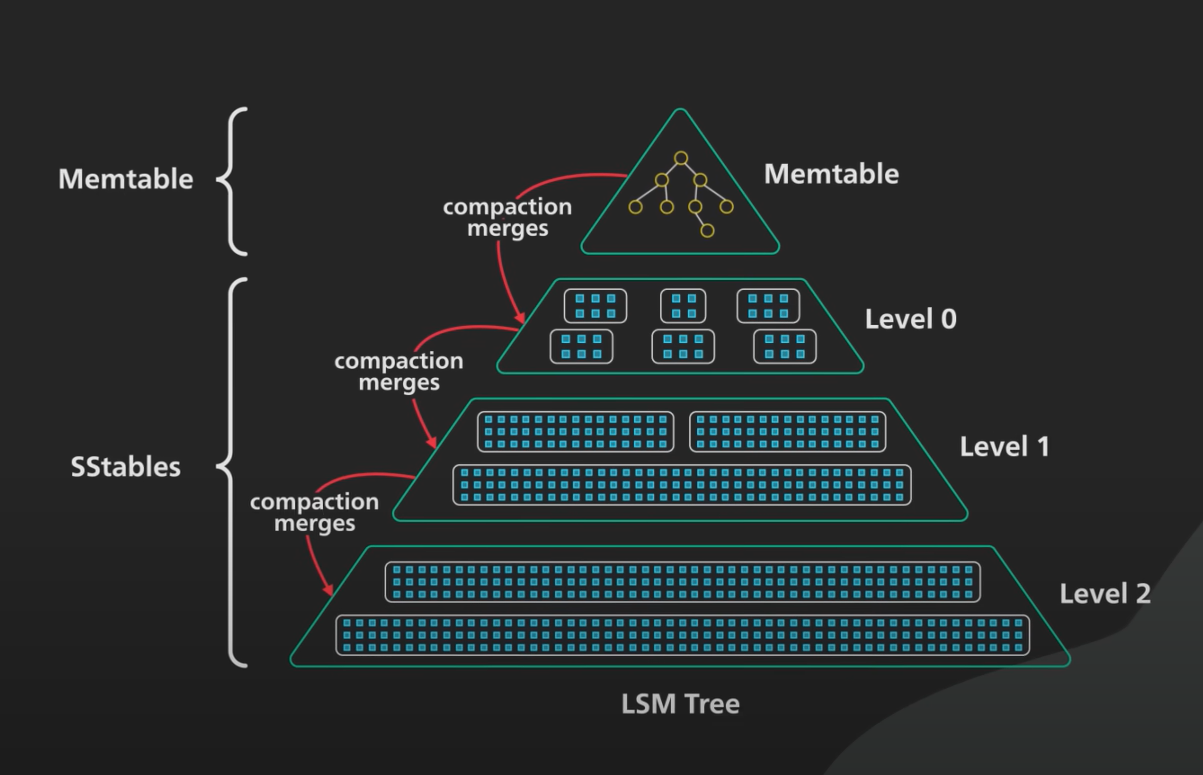
\includegraphics[scale=0.23]{Compaction.png}
    \end{columns} 
    
\end{frame}

\subsection{Simple two levels LS tree}

\begin{frame}
    \frametitle{Two-Level LSM Tree}
    \begin{enumerate}
        \item Simpler version of LSM Tree
        \item One level SSTable
    \end{enumerate}
    \bigskip
    New records are inserted into the Memtable. If the insertion causes the Memtable component to exceed a certain size threshold, a contiguous segment of entries is removed from Memtable and merged into SSTables on disk. 
\end{frame}

\begin{frame}
    \frametitle{Two-Level LSM Tree}
    \begin{center}
         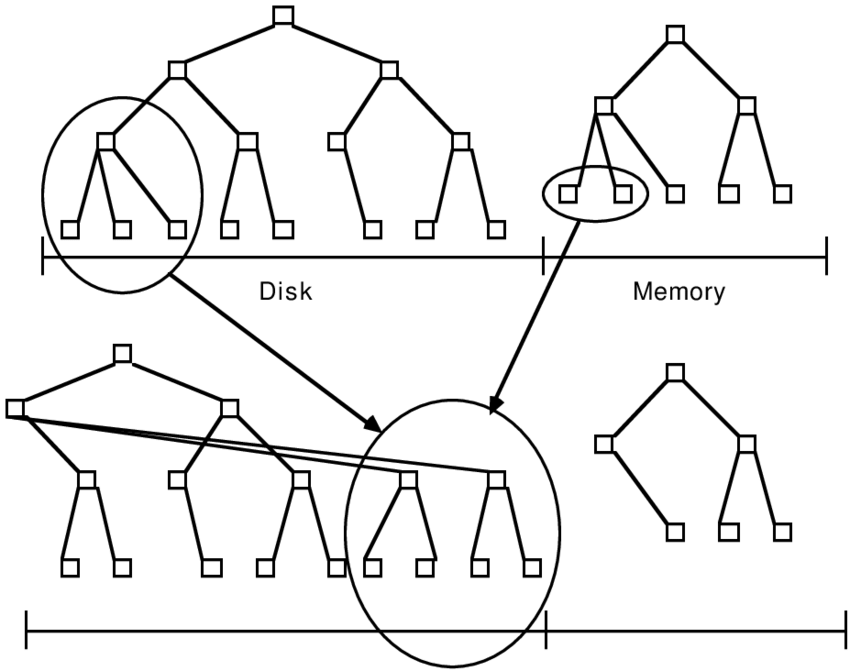
\includegraphics[scale=0.28]{TwoLevelLSM.png}
    \end{center}
\end{frame}

%------------------------------------------------

\section{Algorithm}

\subsection{Process}

\begin{frame}
    \frametitle{Process}
    
    % Define rect styles
    \tikzstyle{circ}=[circle, minimum size=2cm, draw=black, thick, fill=green!50]
    \tikzstyle{rect} = [rectangle, draw, fill=blue!20, node distance=5cm,
    text width=7em, text centered, rounded corners, minimum height=4em, minimum width=8em]
    \tikzstyle{rect2} = [rectangle, draw, fill=yellow!20, node distance=5cm,
    text width=7em, text centered, rounded corners, minimum height=4em, minimum width=12em]
    \tikzstyle{line} = [draw, ->, -latex']
    \tikzstyle{compact} = [draw, ellipse,fill=green!20, node distance=5cm,
    minimum height=2em]
    \tikzstyle{rect3} = [rectangle, draw, fill=blue!40, node distance=2cm,
    text width=2em, text centered, rounded corners, minimum height=2em, minimum width=2em]

    \resizebox{20em}{14em}{
    \begin{center}
        \begin{tikzpicture}[node distance = 2cm, auto]
    
        % Place nodes
        \node [rect] (write) {Write Request};
        \node [rect,  fill=green!50, right of=write] (bf) {Bloom Filter};
        \node [rect, right of=bf] (read) {Read Request};
        \node [circ, below of=read, node distance=4cm] (ret) {Return data};
        \node [rect, below of=bf, fill=yellow!40] (mem) {Memtable};
        \node [rect2, below of=mem] (sstab) {SSTable};
        \node [rect, left of=sstab,fill=red!30] (wal) {WAL};
        \node [rect, right of=sstab,fill=yellow!20] (idx) {Index};
        \node [rect, above of=idx,fill=yellow!20, node distance=3cm] (inmem) {In-memory Index};
        \node[compact, below left of=idx, node distance= 3cm and 5cm] (comp) {Compactor};
        % Draw edges
        \path [line] (write) -- node[above] {(3)} (bf);
        \path [line] (write) -- node[left] {(1)} (wal);
        \path [line] (write) -- node[below left] {(2)} (mem);
        \path [line] (read) -- node[above] {(1)} (bf);
        \path [line] (read) -- node[below right] {(2)} (mem);
        \path [line] (read) -- node[right] {(3)} (ret);
        \path [line, dashed] (mem) -- node[near end] {flush} (sstab);
        \path [line, dashed] (inmem) -- (sstab);
        \path [line, dashed] (idx) -- (inmem);
        \path [line] (comp) to [out=180,in=270] (sstab);
        \path [line] (comp) to [out=0,in=270] (idx);
        \draw (-3,-11) rectangle (13,-9);
        \node [rect3,above left of=wal] (disk) {Disk};
    
\end{tikzpicture}
    \end{center}
}
    
\end{frame}

\subsection{Write}

\begin{frame}
    \frametitle{Write}

    % Define rect styles
    \tikzstyle{circ}=[circle, minimum size=8cm, draw=black, thick, fill=green!50]
\tikzstyle{rect} = [rectangle, draw, fill=blue!20, node distance=5cm,
    text width=7em, text centered, rounded corners, minimum height=4em, minimum width=8em]
\tikzstyle{line} = [draw, ->, -latex']

\resizebox{31em}{14em}{
    \begin{center}
\begin{tikzpicture}
    % Place nodes
    \node [rect, fill=yellow!20] (ser) {Server};
    \node[draw, right of=ser, fill=yellow!50, node distance=6cm] (memt) {
    \begin{minipage}[t][3cm]{3cm}
       \begin{center}
           \textbf{\underline {\large{Memtable}}}
           \begin{enumerate}
               \item Topu, 20
           \end{enumerate}
       \end{center}
    \end{minipage}
};
    \node[circ, right of=memt, fill=blue!30, node distance=7cm] (disk) {
    \begin{minipage}[t][6cm]{6cm}
       \begin{center}
           \textbf{\underline {\Large{Disk}}}\\
       \end{center}
    \end{minipage}
};

    \path [line] (ser) -- node[above] {Write} node[below] {(Topu, 20)} (memt);
    
    
\end{tikzpicture}
    \end{center}
}

\end{frame}

\begin{frame}
    \frametitle{Write}

    % Define rect styles
    \tikzstyle{circ}=[circle, minimum size=8cm, draw=black, thick, fill=green!50]
\tikzstyle{rect} = [rectangle, draw, fill=blue!20, node distance=5cm,
    text width=7em, text centered, rounded corners, minimum height=4em, minimum width=8em]
\tikzstyle{line} = [draw, ->, -latex']

\resizebox{31em}{14em}{
    \begin{center}
\begin{tikzpicture}
    % Place nodes
    \node [rect, fill=yellow!20] (ser) {Server};
    \node[draw, right of=ser, fill=yellow!50, node distance=6cm] (memt) {
    \begin{minipage}[t][3cm]{3cm}
       \begin{center}
           \textbf{\underline {\large{Memtable}}}
           \begin{enumerate}
               \item Rahim, 30
               \item Topu, 20
           \end{enumerate}
       \end{center}
    \end{minipage}
};
    \node[circ, right of=memt, fill=blue!30, node distance=7cm] (disk) {
    \begin{minipage}[t][6cm]{6cm}
       \begin{center}
           \textbf{\underline {\Large{Disk}}}\\
       \end{center}
    \end{minipage}
};

    \path [line] (ser) -- node[above] {Write} node[below] {(Rahim, 30)} (memt);
    
    
\end{tikzpicture}
    \end{center}
}

\end{frame}

\begin{frame}
    \frametitle{Write}

    % Define rect styles
    \tikzstyle{circ}=[circle, minimum size=8cm, draw=black, thick, fill=green!50]
\tikzstyle{rect} = [rectangle, draw, fill=blue!20, node distance=5cm,
    text width=7em, text centered, rounded corners, minimum height=4em, minimum width=8em]
\tikzstyle{line} = [draw, ->, -latex']

\resizebox{31em}{14em}{
    \begin{center}
\begin{tikzpicture}
    % Place nodes
    \node [rect, fill=yellow!20] (ser) {Server};
    \node[draw, right of=ser, fill=yellow!50, node distance=6cm] (memt) {
    \begin{minipage}[t][3cm]{3cm}
       \begin{center}
           \textbf{\underline {\large{Memtable}}}
           \begin{enumerate}
               \item Rahim, 30
               \item Sopu, 10
               \item Topu, 20
           \end{enumerate}
       \end{center}
    \end{minipage}
};
    \node[circ, right of=memt, fill=blue!30, node distance=7cm] (disk) {
    \begin{minipage}[t][6cm]{6cm}
       \begin{center}
           \textbf{\underline {\Large{Disk}}}\\
       \end{center}
    \end{minipage}
};

    \path [line] (ser) -- node[above] {Write} node[below] {(Sopu, 10)} (memt);
    
    
\end{tikzpicture}
    \end{center}
}

\end{frame}

\begin{frame}
    \frametitle{Write}

    % Define rect styles
    \tikzstyle{circ}=[circle, minimum size=8cm, draw=black, thick, fill=green!50]
\tikzstyle{rect} = [rectangle, draw, fill=blue!20, node distance=5cm,
    text width=7em, text centered, rounded corners, minimum height=4em, minimum width=8em]
\tikzstyle{line} = [draw, ->, -latex']

    \begin{center}
\begin{tikzpicture}
    % Place nodes
    \filldraw[color=red!60, fill=blue!30, very thick](0,0) circle (2.8);
    \node[] at (-1,2) {\textbf{Disk}};
    \resizebox{5em}{4em}{
    \node[draw, fill=yellow!50, node distance=6cm] (memt) {
    \begin{minipage}[t][3cm]{3cm}
       \begin{center}
           \textbf{\underline {\large{SSTable}}}
           \begin{enumerate}
               \item Rahim, 30
               \item Sopu, 10
               \item Topu, 20
           \end{enumerate}
       \end{center}
    \end{minipage}
};
}
\end{tikzpicture}
    \end{center}
    \begin{boxD}
After reaching threshold value, memtable is flushed as SSTable into the disk
\end{boxD}
\end{frame}

\begin{frame}
    \frametitle{Write}

    % Define rect styles
    \tikzstyle{circ}=[circle, minimum size=8cm, draw=black, thick, fill=green!50]
\tikzstyle{rect} = [rectangle, draw, fill=blue!20, node distance=5cm,
    text width=7em, text centered, rounded corners, minimum height=4em, minimum width=8em]
\tikzstyle{line} = [draw, ->, -latex']

    \begin{center}
\begin{tikzpicture}
    % Place nodes
    \filldraw[color=red!60, fill=blue!30, very thick](0,0.8) ellipse (5 and 2.8);
    \node[] at (0,2.5) {\textbf{Disk}};
    \resizebox{1em}{1em}{
    \node[draw, fill=yellow!50, node distance=2cm, left of=memt2] (memt1) {
    \begin{minipage}[t][2.5cm]{3cm}
       \begin{center}
           \textbf{\underline {\large{SSTable}}}
           \begin{enumerate}
               \item Rahim, 30
               \item Sopu, 10
               \item Topu, 20
           \end{enumerate}
       \end{center}
    \end{minipage}
};
    \node[draw, fill=yellow!50, right of=memt1, node distance=4cm] (memt2) {
    \begin{minipage}[t][2.5cm]{3cm}
       \begin{center}
           \textbf{\underline {\large{SSTable}}}
           \begin{enumerate}
               \item Jarif, 50
               \item Nolan, 25
               \item Topu, 15
           \end{enumerate}
       \end{center}
    \end{minipage}
};
}
\end{tikzpicture}
    \end{center}
\begin{boxD}
SSTable is immutable. And so the value of key "Topu" is not changed
\end{boxD}
\end{frame}

\begin{frame}
    \frametitle{Compactor}

    % Define rect styles
    \tikzstyle{circ}=[circle, minimum size=8cm, draw=black, thick, fill=green!50]
\tikzstyle{rect} = [rectangle, draw, fill=blue!20, node distance=5cm,
    text width=7em, text centered, rounded corners, minimum height=4em, minimum width=8em]
\tikzstyle{line} = [draw, ->, -latex']

    \begin{center}
\begin{tikzpicture}
    % Place nodes
    \filldraw[color=red!60, fill=blue!30, very thick](0,0.8) ellipse (5 and 2.8);
    \node[] at (0,2.5) {\textbf{Disk}};
    \resizebox{1em}{1em}{
    \node[draw, fill=yellow!50, node distance=1cm] (memt1) {
    \begin{minipage}[t][3.5cm]{3cm}
       \begin{center}
           \textbf{\underline {\large{SSTable}}}
           \begin{enumerate}
               \item Jarif, 50
               \item Nolan, 25
               \item Rahim, 30
               \item Sopu, 10
               \item Topu, 15
           \end{enumerate}
       \end{center}
    \end{minipage}
};
}
\end{tikzpicture}
    \end{center}
\begin{boxD}
Compactor compacts SSTables, removes redundancy
\end{boxD}
\end{frame}

\begin{frame}
    \frametitle{Lose data in system failure!!!}

    \begin{columns} 
        \column{0.7\textwidth}
            We know that MemTable is an in-memory data structure. So if system crashes or a failure occurs then all data inside MemTable is lost!! \newline \newline
            WAL comes to the rescue: 
            \begin{itemize}
                \item Write Ahead Log
                \item Helps to recover lost data
            \end{itemize}
        \column{0.3\textwidth}
            
\includegraphics[scale=0.05]{terrified.png}
    \end{columns}
\end{frame}

\subsection{Read}

\begin{frame}
    \frametitle{Read}

    % Define rect styles
    \tikzstyle{circ}=[circle, minimum size=8cm, draw=black, thick, fill=green!50]
\tikzstyle{rect} = [rectangle, draw, fill=blue!20, node distance=5cm,
    text width=7em, text centered, rounded corners, minimum height=4em, minimum width=8em]
\tikzstyle{line} = [draw, ->, -latex']

\resizebox{31em}{14em}{
    \begin{center}
\begin{tikzpicture}
    % Place nodes
    \node [rect, fill=yellow!20] (ser) {Server};
    \node[draw, right of=ser, fill=yellow!50, node distance=6cm] (memt) {
    \begin{minipage}[t][3cm]{3cm}
       \begin{center}
           \textbf{\underline {\large{Memtable}}}
           \begin{enumerate}
               \item Jamie, 22
               \item Landon, 43
           \end{enumerate}
       \end{center}
    \end{minipage}
};
    \path [line] (ser) -- node[above] {Read} node[below] {(Landon)} (memt);
    \draw[violet] (6,0.1) ellipse (1.3 and 0.4);
\end{tikzpicture}
    \end{center}
}
\begin{boxD}
It first checks the memtable. If found, then returns the data.
\end{boxD}
\end{frame}

\begin{frame}
    \frametitle{Read}

    % Define rect styles
    \tikzstyle{circ}=[circle, minimum size=8cm, draw=black, thick, fill=green!50]
\tikzstyle{rectnow} = [rectangle, draw, fill=blue!20, node distance=3cm,
    text width=2em, text centered, rounded corners, minimum height=2em, minimum width=4em]
\tikzstyle{line} = [draw, ->, -latex']

    \begin{center}
\begin{tikzpicture}
    % Place nodes
    \filldraw[color=red!60, fill=blue!30, very thick](1.5,0) ellipse (5 and 2.8);
    \node[] at (1.5,2.5) {\textbf{Disk}};
    \resizebox{1em}{1em}{
    \node[draw, fill=yellow!50, node distance=2cm, left of=memt2] (memt1) {
    \begin{minipage}[t][3cm]{3cm}
       \begin{center}
           \textbf{\underline {\large{SSTable}}}
           \begin{enumerate}
               \item Rahim, 30
               \item Sopu, 10
               \item Topu, 20
           \end{enumerate}
       \end{center}
    \end{minipage}
};
    \node[draw, fill=yellow!50, right of=memt1, node distance=4cm] (memt2) {
    \begin{minipage}[t][3cm]{3cm}
       \begin{center}
           \textbf{\underline {\large{SSTable}}}
           \begin{enumerate}
               \item Jarif, 50
               \item Nolan, 25
               \item Topu, 15
           \end{enumerate}
       \end{center}
    \end{minipage}
};
}
\end{tikzpicture}
    \end{center}
\begin{boxD}
After checking memtable, it checks all the SSTables
\end{boxD}
\end{frame}

\begin{frame}
    \frametitle{Check All The SSTables? (nLogn)}
    \begin{columns} 
        \column{0.7\textwidth}
            If the data we are searching for is not there in the memtable nor in the SSTables, then? Time for searching all the SSTables go in vain! \newline \newline
            Bloom filter is there for us: 
            \begin{itemize}
                \item Probabilistic data structure
                \item Return values to tell us whether the data exists or not
            \end{itemize}
        \column{0.3\textwidth}
            
\includegraphics[scale=0.2]{surprise.jpg}
    \end{columns}
\end{frame}


\setbeamercovered{transparent}
\begin{frame}{Bloom filter?
\includegraphics[width=0.05\textwidth]{emoji_thinks.png}}
\begin{itemize}
    \item use a set of hash functions to create a bit vector\pause
    \item used 3 hash functions in the example
    \end{itemize}
    \tikzstyle{bit} = [rectangle, draw, minimum size=1cm]
  \tikzstyle{word} = [circle, draw, minimum size=1cm]
  \begin{tikzpicture}
  
  % Bloom filter bits
  \foreach \i in {0,1,2,3,...,10}
    \node[bit] at (\i,0) (b\i) {};
  \foreach \i in {0,1,2,3,...,10}
    \node[below] at (b\i.south){\i};
    \foreach \i in {0,5,10}
     \node[center] at (\i,0){\textcolor{green}{1}};
   \foreach \i in {1,2,3,4,6,7,8,9}
     \node[center] at (\i,0){\textcolor{red}{0}};
     
  % Word to check
  \node[word] at (-1,0) (w) {27};
  \node[below] at (w.south) {\textbf{index}};
  % Hash functions
  \node[above] at (b0.north) {27\%27};
  \node[above] at (b5.north) {27\%11};
  \node[above] at (b10.north) {27\%17};
  
  % Arrows indicating hash values
  \draw[->] (w.east) to[bend left] (b0.north);
  \draw[->] (w.east) to[bend left=20] (b5.north);
  \draw[->] (w.east) to[bend right] (b10.north);
  
\end{tikzpicture}
\begin{itemize}
    \item \pause When a new element is added to the Bloom filter, it is hashed by each of the hash functions, and the corresponding bits in the bit vector are set to 1.
    
  \end{itemize}
    
\end{frame}

\begin{frame}
    \frametitle{Bloom Filter}
    \tikzstyle{rect} = [rectangle, draw, fill=blue!20, node distance=3cm,
    text width=7em, text centered, rounded corners, minimum height=4em, minimum width=8em]
    \tikzstyle{line} = [draw, ->, -latex']
        \begin{center}
            
        \begin{tikzpicture}[auto]
    
        % Place nodes
        \node [rect] (bf) at (0,1) {Bloom Filter};
        \node [rect] (0) at (5,3) {Data doesn't exist};
        \node [rect] (1) at (5,-1) {Data may or may not exist};
        
        % Draw edges
        \path [line] (bf) -- node[above left] {returns 0} (0);
        \path [line] (bf) -- node[below left] {returns 1} (1);
    
\end{tikzpicture}
\begin{boxD}
Complexity = $O(c) + pO(n)$
\end{boxD}
\end{center}

\end{frame}
\subsection{Complexity}

\begin{frame}
    \frametitle{Complexity}
    \begin{table}[h!]
        \centering
        \begin{tabular}{|c|c|c|}
            \hline
           Action  &  Best Case & Worst Case\\
           \hline
           Write  & $O(1)$ & $O(1)$ \\
           Read  & $O(1)$ & $O(nlogn)$\\
           \hline
        \end{tabular}
        \caption{Time Complexities of LSM Tree}
        \label{tab:my_label}
    \end{table}
    \begin{boxD}
After using Bloom filter, read complexity = $O(c) + pO(n)$
\end{boxD}
\end{frame}

%------------------------------------------------

\section{Advantages \& Disadvantages}
\begin{frame}
  \frametitle{Advantages}

  \begin{itemize}
    \item Fast write performance \pause
    \begin{itemize}
      \item written to a memory buffer \pause
    \end{itemize}
    \item Storage efficiency \pause
    \begin{itemize}
      \item merging and compaction \pause
    \end{itemize}
    \item What happens when size of the dataset grows? 
\includegraphics[width=0.05\textwidth]{emoji_thinks.png}
    
  \end{itemize}

\end{frame}


\begin{frame}
  \frametitle{Disadvantages}

  \begin{itemize}
    \item Higher read latency \pause
    \begin{itemize}
      \item data is stored across multiple levels \pause
    \end{itemize}
    \item complexity? 
\includegraphics[width=0.05\textwidth]{emoji_thinks.png} \pause
    \item size of the datasets \pause
    \begin{itemize}
      \item large datasets 



     \item smaller datasets? \pause
    \end{itemize}
    \item memory requirements 
    \begin{itemize}
      \item require more memory \pause
      due to their use of a memory buffer and multiple levels
    \end{itemize}
  \end{itemize}

\end{frame}







%------------------------------------------------

\section{Conclusion}


\begin{frame}{References} 
    \begin{figure}
        \begin{itemize}
            \item[] 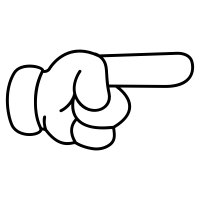
\includegraphics[scale=0.1]{indicator.png} \href{https://www.cs.umb.edu/~poneil/lsmtree.pdf}{University of Massachusetts Boston}
            \item[] 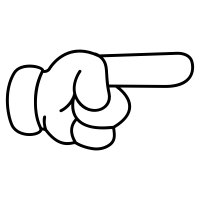
\includegraphics[scale=0.1]{indicator.png}  \href{https://en.wikipedia.org/wiki/Log-structured_merge-tree}{Wikipedia}
        \end{itemize}
    \end{figure}{}
\end{frame}{}

\end{document} 